\documentclass[conference]{IEEEtran}
\usepackage[T1]{fontenc}
\usepackage[utf8]{inputenc}
\usepackage{helvet}
\usepackage{courier}
\usepackage{amssymb}
\usepackage{xcolor}
\usepackage{array}
\usepackage{booktabs}
\usepackage{graphicx}
\usepackage{tikz}
\usetikzlibrary{shapes.geometric,arrows.meta,positioning,fit,backgrounds,calc}
\usepackage{listings}
\usepackage{cite}
\usepackage{microtype}
\usepackage{url}
\setlength{\textfloatsep}{8pt plus 2pt minus 2pt}
\setlength{\dbltextfloatsep}{8pt plus 2pt minus 2pt}
\setlength{\floatsep}{7pt plus 2pt minus 2pt}

% ==== figure palette: three hues plus greys, separated by value in greyscale
\definecolor{agF}{HTML}{F6F2FC}\definecolor{agB}{HTML}{6B4FA0} % agent, violet
\definecolor{rbF}{HTML}{A9C4DC}\definecolor{rbB}{HTML}{2F6FAF} % apparatus, blue
\definecolor{dsF}{HTML}{DCDCE0}\definecolor{dsB}{HTML}{9A9AA0} % the log, grey
\definecolor{hgB}{HTML}{3E6B52}                                % the decider, green
\definecolor{dgrey}{HTML}{555555}\definecolor{fgrey}{HTML}{7A7A7A}

% ==== code: the same fonts, no frame, a hair rule above and below
\lstset{basicstyle=\ttfamily\fontsize{6.4}{7.4}\selectfont, columns=fullflexible, keepspaces=true,
  language=Python, commentstyle=\color{fgrey}, keywordstyle=\bfseries, showstringspaces=false,
  aboveskip=3pt, belowskip=2pt, xleftmargin=0pt, xrightmargin=1pt, frame=lines, framerule=0.3pt, rulecolor=\color{black!40},
  breaklines=true, breakatwhitespace=true, breakindent=8pt, captionpos=b, abovecaptionskip=3pt, belowcaptionskip=0pt}

\begin{document}

\title{Constrained Cache Design by a Council of Agents:\\A CHIA Loop That Measures and Gates Itself}

\author{}

\maketitle

\begin{abstract}
Choosing a cache hierarchy means setting the sets, ways, prefetcher, replacement policy and queue
depth of every level at once, under a silicon budget and a power budget, with one simulation per
design to judge it. We search 13 such knobs of a three-level hierarchy, 6.6 million designs,
under area and power constraints of 4.0\,mm$^2$ and 1.0\,W, with a council of Gemini agents
built as a CHIA loop: an analyst that diagnoses the current design, four specialists that each
propose one move, a statistician with a Gaussian process, and a repair that shrinks a design that
violated the power constraint. The council reaches the quality that random search attains after
1000 designs in 39 to 44 designs, 23 to 25 times fewer simulations. % results/ledgers/lean/*lean20* (council), *random* (random); council_loop/demo.py section 3
CHIA provided the nodes, the cluster and the profiler; we added what the loop needed and CHIA
lacked: a Gemini node that bills thinking tokens, a ChampSim node that builds a whole hierarchy,
an evaluation ledger, a spend view over the profiler log, and two gates in which a cheap
calibrated decider judges which agent calls and which briefing sections are worth paying for.
Applied, the gates reach the same final IPC for 22 to 30\% results/report/lean20*/gating.md; council_loop/demo.py section 2
The blocks travel: on CHIA's own CIRCT loop, the call gate cuts the assess stage from 16 to 13
agent turns while sending the same issues forward. % results/audit/circt_assess/README.md
Every table reproduces from the repository with one command and no API key.
\end{abstract}

% =====================================================================
\section{Introduction}
A cache hierarchy is usually set by sweeps and experience: one level at a time, one knob at a
time, the rest held fixed. The knobs, however, do not act independently. A larger last level
costs power that a smaller second level could have saved, a prefetcher that helps one level floods
the next, and a constraint on silicon or power turns every gain into a trade-off. Since each
design costs a simulation, the currency of the search is the number of designs measured.

CHIA \cite{chia} is a framework for building loops in which agents propose and tools measure,
with every step a task on a cluster and a profiler recording it. We built such a loop for this
problem: a council of agents that reads the simulator's counters, diagnoses where the time and
the power go, proposes designs and has them measured five at a time. Against random search over
the same feasible space, the council reaches the quality that random search attains after 1000
designs in 39 to 44 designs, both under the constraints and without them. % results/ledgers/lean/*lean20*, *random*; council_loop/demo.py section 3

Such loops are usually judged by that result alone, which says nothing about what the loop
cost or where. The CHIA paper \cite{chia} names the gap: ``data collection and profiling of both
results and of the loop itself built in as first-class citizens''. % CHIA paper, section 2
We followed that principle throughout. The loop's model calls, builds, simulations, candidates
and gate decisions are all CHIA tasks, so one profiler log per run holds all of them, and the
blocks we added either read that log or add events to it: a spend view that sums the log per
node and model, a ledger that scores every candidate the way search methods are compared, and two
gates in which a cheap calibrated decider answers one yes-or-no question before an optional agent
call or for each section of a briefing. Run in shadow, the gates only record; this showed that
57\% of the specialists' calls ended in a hold, and which of them a decider could have foreseen.
Applied, the gates gave the same final IPC for 22 to 30\% results/vm2/results/skip_gate.jsonl; results/report/lean20*/gating.md

Sections~\ref{sec:problem} to \ref{sec:artifact} follow that order: the design problem, the
council as a CHIA loop, the result against random search, the cost and the gates, the blocks on
CHIA's own CIRCT loop, what the instruments found, and the artifact.

% =====================================================================
\section{The Design Problem}\label{sec:problem}
The chip is ChampSim's \cite{champsim} stock core widened to 6-wide issue with a 384-entry
reorder buffer, at 3.8\,GHz in 22\,nm, with DDR5-4800 over two channels. % council_loop/socs.py (next)
The search moves 13 knobs: the sets and ways of the L1D, L2 and LLC on per-level ladders, the
prefetcher of each level, the replacement policy of the L2 and LLC, and the miss-handling depth of
both, 6.6 million designs in all. Two constraints make this a design problem rather than a sweep:
4.0\,mm$^2$ of cache silicon and 1.0\,W of cache plus off-chip power, and a design may not run
the workload slower than the stock chip does. The two constraints become known at
different times, and that shapes the loop. Silicon and leakage come from CACTI~7 \cite{cacti7} at
22\,nm and are known before a design is simulated, so a design that exceeds the area constraint is
never run. Power is CACTI's energies times the simulator's hit and miss counters plus 15\,pJ per
bit moved off chip, so it is known only afterwards: a design that exceeds the power constraint is
measured and read by the agents, but never becomes the incumbent. % council_loop/space.py power_split
The stock chip itself draws 1.095\,W on the workload and thus exceeds the power constraint, so
the reference is the stock with its LLC halved: 1.96\,mm$^2$, 0.805\,W, IPC 0.935. The
constraints are binding: 36\% of the council's candidates were refused after measurement, 21\% by
power and 19\% by the speed floor, some by both. The area constraint rarely binds, since good
designs are small; the best draws 0.67\,W on 1.33\,mm$^2$. A second regime drops both
constraints. % results/ledgers/lean/next_llama2_lean20_cap*

The workload is the llama2 inference trace of the ChampSim ML suite, simulated at 1M warm-up and
2M instructions; 40 designs re-measured at 5M/25M rank the same (Spearman 0.986, top-5 overlap
80\%). % results/vm2/results/fidelity_llama2.json
We chose the most demanding of six ML traces deliberately, the one with the most headroom over
the stock and the deepest coupling between knobs, so that the council is tested where a sweep
fails. % council_loop/search.py gate, run over the six traces

% =====================================================================
\section{The Council as a CHIA Loop}\label{sec:council}
\textbf{One round.} Fig.~\ref{fig:loop} shows one round. Round one measures the analyst's opening
design and 19 random feasible designs. Every later round measures one wave of five. A
statistician, a Gaussian process over every design this run has measured, proposes its top pick;
the analyst writes a sheet (a verdict per level with its evidence, the knobs that failed alone,
the headroom under each constraint) and one whole design; four specialists, for prefetching,
geometry, replacement and concurrency, each propose one move on their own knobs or hold. The wave
takes at most five, in this order: the statistician's pick, the analyst's design, a gain refused
last round by the power constraint and shrunk to fit, the specialists' moves, and untried
single-knob moves at the level the sheet blames, to fill what is left. The incumbent is the best
feasible design measured, whoever proposed it, and a move already measured against it counts as
a hold. One model serves every call, Gemini~3.1~Pro on Vertex at temperature 0.7 with a thinking
budget of 4096 tokens. % council_loop/council.py, council_loop/analyst.py

\begin{figure}[!t]
\centering
\resizebox{0.95\columnwidth}{!}{% fig-loop.tex -- single-column figure: one round of the council. The agents in a dashed group (violet,
% tasks of the Gemini node), the decider's gate as a diamond (green), the apparatus beneath (blue, CHIA's
% ChampSim nodes and the ledger); the round closes from the ledger back to the agents.
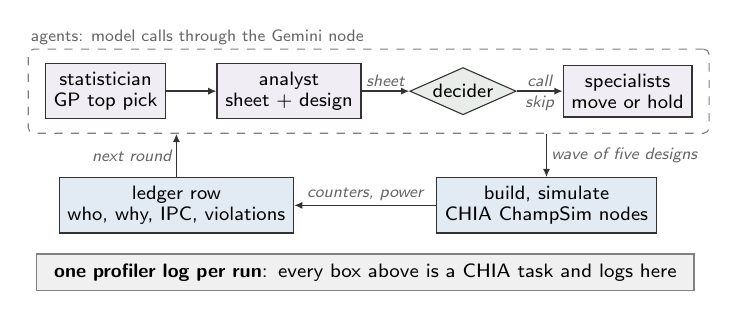
\begin{tikzpicture}[x=1cm,y=1cm, font=\sffamily\fontsize{6.8}{7.8}\selectfont,
  box/.style={draw=black!80, line width=0.4pt, align=center, inner sep=3pt, minimum height=0.6cm},
  agent/.style={box, fill=agB!10},
  tool/.style={box, fill=rbB!14},
  gate/.style={diamond, aspect=2.2, draw=black!80, line width=0.4pt, fill=hgB!12, inner sep=0pt,
               minimum width=1.35cm, minimum height=0.6cm},
  group/.style={draw=black!50, dashed, line width=0.4pt, rounded corners=2pt, inner xsep=6pt, inner ysep=5pt},
  grouplabel/.style={font=\sffamily\fontsize{6.2}{7}\selectfont, text=black!60, anchor=south west, inner sep=1pt},
  arr/.style={-{Latex[length=3pt,width=2.6pt]}, line width=0.5pt, draw=black!80},
  lab/.style={font=\sffamily\fontsize{6.2}{7}\selectfont\itshape, text=black!60, inner sep=1.5pt, align=center},
  ]
% ---- the agents
\node[agent] (stat) at (1.00,3.0) {statistician\\GP top pick};
\node[agent] (anal) at (3.33,3.0) {analyst\\sheet + design};
\node[gate]  (gate) at (5.54,3.0) {decider};
\node[agent] (spec) at (7.63,3.0) {specialists\\move or hold};
\draw[arr] (stat) -- (anal);
\draw[arr] (anal) -- node[lab, above] {sheet} (gate);
\draw[arr] (gate) -- node[lab, above] {call} node[lab, below] {skip} (spec);
\begin{scope}[on background layer]
  \node[group, fit=(stat)(anal)(gate)(spec)] (agents) {};
\end{scope}
\node[grouplabel] at (agents.north west) {agents: model calls through the Gemini node};
% ---- the apparatus, and the round
\node[tool] (sim) at (6.6,1.55) {build, simulate\\CHIA ChampSim nodes};
\node[tool] (led) at (1.9,1.55) {ledger row\\who, why, IPC, violations};
\draw[arr] (agents.south -| sim) -- node[lab, right] {wave of five designs} (sim);
\draw[arr] (sim) -- node[lab, above] {counters, power} (led);
\draw[arr] (led) -- node[lab, left] {next round} (agents.south -| led);
% ---- the log
\node[draw=black!50, fill=black!6, line width=0.4pt, align=center, inner sep=3.5pt, text width=8.1cm] at (4.3,0.7)
  {\textbf{one profiler log per run}: every box above is a CHIA task and logs here};
\end{tikzpicture}
}
\caption{One round of the council. Violet: the agents, tasks of the Gemini node; blue: the
apparatus, CHIA's ChampSim nodes and the ledger; green: the decider's gate. Every box is a CHIA
task.}
\label{fig:loop}
\end{figure}

\textbf{What CHIA gave and what we added.} Every box in Fig.~\ref{fig:loop} is a CHIA task on a
Ray \cite{ray} cluster. Each run connects under its own name with its own profiler collector, so
a run's log is a complete record of it, and simulations run through CHIA's own ChampSim run node.
Three nodes did not exist, and we wrote them in CHIA's layout. CHIA's Vertex node drives a tool
loop under a fixed generation config and leaves the thinking tokens out of its usage record,
whereas our Gemini node makes one JSON call at a set temperature and thinking budget and records
every token, the cost in dollars and the caller. CHIA's build node writes one prefetcher at one
level, whereas ours builds from a whole configuration. CHIA's run node keeps a subset of the
simulator's record, less than the analyst reads, so a 7-line patch returns the whole of it, and
the loop's parse gives identical numbers. % remeasure_check: 103 metrics equal
Every design measured is one ledger row and one \texttt{candidate} event in the log.

\textbf{Protocol.} The budget unit is a design: wall time at this fidelity shows no advantage
either way, since the model's minute per round offsets the fewer rounds. Random search draws 1000
feasible designs over three seeds; the council runs 60 designs, or 20 without a new incumbent,
with four seeds per arm and regime. The target is the mean over random's seeds of its best after
1000 designs; a seed that spends its budget under the target counts at the budget, 60 designs,
with its final IPC beside it. Every arm is scored from the same ledger rows, random's
being rebuilt from its seed and the result table. % council_loop/search.py, council_loop/ledgers.py

% =====================================================================
\section{Against Random Search}\label{sec:random}

\begin{table}[!t]
\caption{The council against random search, means over seeds. The target is random's mean best
IPC after 1000 designs; a council seed under it at the budget counts as 60 designs. New bests: who
proposed the new incumbents}
\label{tab:random}
\centering
\scriptsize
\renewcommand{\arraystretch}{0.95}
\setlength{\tabcolsep}{3.5pt}
\begin{tabular}{@{}lcccccc@{}}
\toprule
 & \textbf{target} & \textbf{council designs} & \textbf{fewer} & \multicolumn{3}{c}{\textbf{new bests found by}} \\
\cmidrule(lr){5-7}
 & \textbf{IPC} & \textbf{to the target} & \textbf{simulations} & model & statistician & fills \\
\midrule
% results/ledgers/lean/*lean20* (source field), *random*; council_loop/demo.py section 3
constrained & 1.4329 & 44 & 23$\times$ & 62\% & 25\% & 13\% \\
unconstrained & 1.5001 & 39 & 25$\times$ & 40\% & 36\% & 24\% \\
\bottomrule
\end{tabular}
\end{table}

\begin{figure}[!t]
\centering
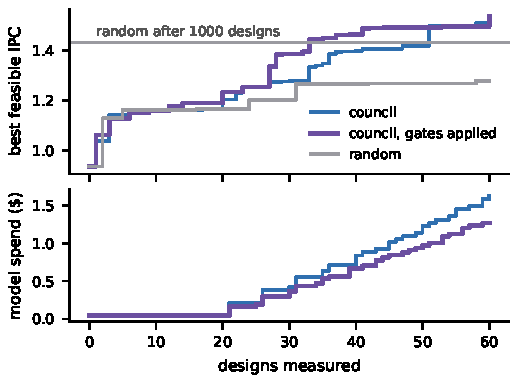
\includegraphics[width=\columnwidth]{fig_curves.pdf}
\caption{Constrained regime, means over seeds: the best feasible IPC as designs are measured, and
the cumulative model spend of the two council arms beneath it. Random's line is its 1000-design
mean.}
\label{fig:curves}
\end{figure}

\textbf{The result.} Random search (Table~\ref{tab:random}, Fig.~\ref{fig:curves}) climbs early,
because a fifth of the feasible space beats the halved stock, and then stalls. The council passes
random's 1000-design quality at 44 designs under the constraints and at 39 without. Fifteen of
its sixteen runs end above that quality; the remaining one ends at 1.497 against 1.5001. % results/ledgers/lean/*lean20*, *random*; council_loop/demo.py section 3

\textbf{Who found the improvements.} The ledger records who proposed every new best design, and
the answer differs between the two regimes. Under the constraints, the model produced most of
them: its whole designs and its repairs of refused gains account for 62\% of the new bests, the
statistician for 25\% and the single-knob fills for 13\%. Unconstrained, the statistician led
with 36\% results/ledgers/lean/*lean20*, the source field of each new best

\textbf{Why.} A constraint makes the objective discontinuous. A design can be faster and still be
refused, and a surrogate fitted to IPC does not see that wall, whereas a model that reads the
counters does, and can say which level to shrink. Without the constraints the landscape is
smooth, and the surrogate's interpolation is the better predictor. The constraints therefore
decide who wins, not whether the search wins, and a ledger that records who won tells the two
apart for each problem.

\textbf{Against Bayesian optimisation.} We also ran a standard Bayesian optimisation, a
random-forest surrogate with expected improvement and the same waves of five, two seeds per
regime. It needs as many designs as the council to reach random's 1000-design quality. Without
the constraints it ends 1\% above the council's final IPC; under them it ends 1\% below the
council and 2.5\% below the gated council, and half to two thirds of its designs came back in
violation of the power constraint, against a third of the council's.
% results/ledgers/lean/next_llama2_bo_cap_bo_s*, nocap_llama2_nocap_bo_bo_s*; best at 60 designs
The same pattern holds: a surrogate predicts well on a smooth landscape, and where the constraint
turns a faster design into an infeasible one, an agent that reads the counters does better.

% =====================================================================
\section{Cheaper at the Same IPC}\label{sec:gates}
\textbf{What the instruments showed.} A run's model bill is \$1.6 to \$1.7; what scales is the
share saved, with more seeds, full fidelity, bigger loops, and every loop in which most optional
calls end in a hold. The recipe above is the sixth version of the council, and the ledger
determined most of what it contains: its rows showed that four rules of earlier versions never
paid and that one setting stalled half the seeds. % council_loop/council.py; results/ledgers/lean/ (the 10-opening runs)
The per-call rows, priced by the spend block, showed what the bill was made of: input 49\%,
thinking 37\% results/vm2/results/llm_calls.jsonl, priced by the spend block
The specialists' rows showed that 57\% of their calls ended in a hold. % results/vm2/results/skip_gate.jsonl
Two levers therefore remained: the calls that end in a hold, and the briefing every call carries.

\textbf{The gate.} A gate in front of a call needs a verdict that is cheap, fast and calibrated,
not a second agent. TypeSafe's Jev \cite{typesafe} answers a typed yes-or-no question with a
probability, at \$0.042 per million input tokens; a round of four questions costs about a tenth
of a cent and returns within a second. % council_loop/council.py (thresholds); results/vm2/results/skip_gate.jsonl
The call gate asks, per specialist and round, whether the analyst's sheet gives evidence for
moving that concern's knobs; Listing~\ref{lst:gate} is the whole of it. The context gate asks,
per section of a briefing, whether the task needs it, judging from the caller's one-line
description of the section, and also rates the task's difficulty, which sets the thinking
budget. Both gates have two modes. In shadow, every call is still made and the verdict is
recorded beside what the call then produced; in apply, the calls under the threshold are not made
and the sections rated unneeded are dropped. The pair is the point: shadow prices the gate before
apply collects the saving, so nothing is skipped on faith.

\begin{lstlisting}[caption={The call gate in front of the council's specialists. The state and the questions belong to the loop, the rest to the block; \texttt{ask\_specialist} is one task of the Gemini node.},label={lst:gate},float=t]
gate = CallGate(JevDecider(), threshold=0.4, mode="apply")
state = {"sheet": sheet_text(sheet)[:2500],
         "current_design": knobs_text(incumbent),
         "statistician_expects": expects[:800]}
questions = {}
for name in CONCERNS:   # prefetch, geometry, replacement, ...
    questions[name] = {
        "instructions": f"Does the sheet give evidence "
                        f"for moving the {name} knobs?",
        "criteria": {"true": "its findings point here",
                     "false": "nothing does; a hold is free"}}
verdicts = gate_and_log(gate, state, questions, label=round)
for name in verdicts:       # shadow: every call made
    if verdicts[name]["consult"]:
        ask_specialist(name)   # apply: the rest not called
\end{lstlisting}

\begin{table}[!t]
\caption{The call gate in shadow over 304 specialist calls of eight runs (gains lost: skipped
proposals that gained more than 0.005 IPC), then both gates applied, 4 seeds per arm and regime}
\label{tab:gate}
\centering
\scriptsize
\renewcommand{\arraystretch}{0.92}
\begin{tabular}{@{}lcccc@{}}
\toprule
\multicolumn{5}{@{}l}{\textit{Shadow: what the gate would have skipped}}\\
threshold & skipped & holds & proposals & gains lost \\
\midrule
% results/vm2/results/skip_gate.jsonl; council_loop/demo.py section 2
0.3 & 93 (31\%) & 68 & 25 & 2 \\
0.4 & 121 (40\%) & 92 & 29 & 2 \\
0.5 & 147 (48\%) & 112 & 35 & 3 \\
\addlinespace[3pt]
\multicolumn{5}{@{}l}{\textit{Applied at 0.4, with the context gate; ``all calls'' is the ungated baseline}}\\
 & \multicolumn{2}{c}{\textbf{constrained}} & \multicolumn{2}{c}{\textbf{unconstrained}} \\
\cmidrule(lr){2-3}\cmidrule(lr){4-5}
 & all calls & gated & all calls & gated \\
\midrule
% results/vm2/results/skip_gate.jsonl, llm_calls.jsonl; results/report/lean20*/; council_loop/demo.py section 2
model spend per run (\$) & 1.63 & 1.27 & 1.71 & 1.20 \\
model calls per run & 47.2 & 34.0 & 49.8 & 31.0 \\
final IPC, mean of seeds & 1.512 & 1.537 & 1.521 & 1.513 \\
less model spend & \multicolumn{2}{c}{22\%} & \multicolumn{2}{c}{30\%} \\
\bottomrule
\end{tabular}
\end{table}

\textbf{What the shadow showed, and what applying it saved.} Table~\ref{tab:gate}: over the 304
specialist calls of the eight shadow runs, a threshold of 0.4 would have skipped 40\%, 92 holds
and 29 proposals, of which two gained more than 0.005 IPC; of the 20 gains above 0.005
among all 304 calls, 18 carried a verdict of 0.4 or more. The context gate drops 16 to 17\% of
the briefing tokens once shown a description per section; shown the sections' first characters
instead, it had rated the evidence unneeded, a negative result we report. % results/vm2/results/skip_gate.jsonl, context_gate.jsonl; results/report/lean20*/gating.md
Applied together, with a specialist's thinking budget reduced when its task is not rated hard,
the council consulted 2.4 to 2.8 specialists a round instead of four and reached the same final
IPC for 22\% less model spend under the constraints and 30\% without (Fig.~\ref{fig:curves}), the
decider's cost included. Nearly all of the saving, 94 to 98\% of it, comes from the calls not
made. The trimmed briefings cut a specialist call's input by 7 to 12\%, but the cost of a call
made was flat, since thinking and answer lengths vary by more than that. % results/vm2/results/llm_calls.jsonl

% =====================================================================
\section{The Blocks Travel}\label{sec:blocks}
Everything the loop needed is a module and a test in CHIA's tree (Table~\ref{tab:blocks}),
installed into the released package by one script; the tests pass inside it, and the CLI's new
format sums a log that CHIA's own Vertex node wrote.

\begin{table}[!t]
\caption{The blocks, what each reads or records, and where each was proven}
\label{tab:blocks}
\centering
\scriptsize
\renewcommand{\arraystretch}{0.92}
\begin{tabular}{@{}>{\raggedright\arraybackslash}p{1.35cm}@{\hspace{4pt}}>{\raggedright\arraybackslash}p{4.55cm}@{\hspace{4pt}}>{\raggedright\arraybackslash}p{2.15cm}@{}}
\toprule
\textbf{Block} & \textbf{What it reads or records} & \textbf{Proven on} \\
\midrule
Spend view and limit &
Dollars and tokens by kind per node and model, from the events. \texttt{chia viz-profile --format
spend}; \texttt{LLMSpend} stops a loop at a spend limit. &
CHIA's Vertex node under a local Ray; the CIRCT stage; the council's own log \\
\addlinespace[2pt]
Evaluation ledger &
One row per candidate: who, why, what it measured, which constraints it violated. From the rows:
best-so-far, evaluations to a target, plateau, speedups, rank agreement. &
Every arm of Sec.~\ref{sec:random} \\
\addlinespace[2pt]
Decider and call gate &
One yes-or-no question per optional call, answered by Jev from the caller's state; shadow
records, apply skips. &
The council (Sec.~\ref{sec:gates}); CIRCT: 16 to 13 turns \\
\addlinespace[2pt]
Context gate &
Per briefing section, the decider judges the caller's one-line description; it also rates the
task's difficulty, which sets the thinking budget. &
The council: 16--17\% fewer briefing tokens \\
\addlinespace[2pt]
Gemini JSON node &
One JSON answer at a set temperature and thinking budget; the event carries every token kind,
the cost in dollars and the caller. &
Every model call of the council \\
\addlinespace[2pt]
ChampSim configuration build &
Builds ChampSim from a whole configuration and returns CHIA's own build result. A 7-line patch
returns the simulator's raw record. &
Every build and run of the council; IPC equal to the loop's own build \\
\bottomrule
\end{tabular}
\end{table}

\textbf{On CHIA's own loop.} CHIA's CIRCT issue solver begins with an \emph{assess} turn, in
which an agent reads a GitHub issue and decides whether it is a bug with one clear fix; an issue
that is not a bug is set aside after that turn, so it still costs the turn. We re-ran the turn
under the blocks: the paper's own prompt, the 16 issues of its Table~5, CHIA's Vertex node under
CHIA's profiler, and the call gate asking the decider ``does this issue report a defect?'' before
the turn, at 0.65. Table~\ref{tab:circt} gives means over passes, since answers vary. The gate
skipped the same three of the five non-bugs in both gated passes and none of the eleven bugs, so
the paper's seven issues proceed to reproduction as before, while turns and tokens fell 19\% and
the decider's 16 decisions cost \$0.0008. % circt README; demo 1
The saving is bounded by the share of non-bugs in the stream, five of sixteen here; what the gate
buys is that the expensive turn is spent only where it is needed, with no bug lost.

\begin{table}[!t]
\caption{CHIA's assess stage over the paper's 16 issues (11 bugs, 5 not), ungated and gated.
Agree: verdicts matching the paper's, of 16. Tokens and dollars: the spend view over each pass's
profiler log}
\label{tab:circt}
\centering
\scriptsize
\renewcommand{\arraystretch}{0.92}
\begin{tabular}{@{}l@{\hspace{5pt}}c@{\hspace{5pt}}c@{\hspace{5pt}}c@{\hspace{5pt}}c@{\hspace{5pt}}c@{\hspace{5pt}}r@{}}
\toprule
 & \textbf{turns} & \textbf{agree} & \multicolumn{2}{c}{\textbf{skipped}} & \textbf{tokens} & \textbf{\$} \\
\cmidrule(lr){4-5}
 & & /16 & bugs & non-bugs & & \\
\midrule
% council_loop/demo.py section 1: verdicts_*.jsonl and <pass>/ChiaProfileCollector.log
ungated, 3 passes & 16 & 14.3 & 0 of 11 & 0 of 5 & 37.7k & 0.095 \\
gated at 0.65, 2 passes & 13 & 14.5 & 0 of 11 & 3 of 5 & 30.4k & 0.081 \\
change & $-$19\% & & & & $-$19\% & $-$15\% \\
\bottomrule
\end{tabular}
\end{table}

\textbf{Six pull requests to CHIA.} What the loop revealed about CHIA's nodes went upstream as
six pull requests, open at the time of writing. Four concern the Vertex node: a prompt that
mentions an undeclared tool made it return success with an empty answer (14 of 16 issues came
back blank); its usage record left out the thinking tokens; a rate
limit raised at once, so a batch died on the first 429; and its generation settings could not be
set per request. One resets the profiler when a collector starts and flushes it when it stops,
so a driver that restarts the collector keeps its events. The sixth returns the ChampSim run
node's raw record, which had kept the first DRAM channel only and no merged misses. % UPSTREAM.md; upstream/README.md

% =====================================================================
\section{What the Instruments Found}\label{sec:found}
\textbf{The model alone does not search.} Without the statistician, the repairs and the fills,
the specialists ran out of proposals at 25 to 28 designs, and the runs ended at IPC 1.15 to 1.17
in both regimes. % results/ledgers/lean/*bare*
\textbf{Grounding is a gauge, not a filter.} Asked whether the sheet supports each of 377
proposals, the decider's verdict did not predict which of them gained, so it measures prompt
discipline and should not be used to skip calls. % results/audit/grounding.jsonl; council_loop/audit.py
\textbf{The decider cannot judge ``one clear fix''} (10 of 11 CIRCT bugs were rated unclear),
which is why the gate asks the narrower question. % results/audit/circt_assess/

% =====================================================================
\section{Artifact, Related Work and Limitations}\label{sec:artifact}
\textbf{Artifact.} \texttt{python3 council\_loop/demo.py} replays every table of this paper from
the shipped records in under a second, with no key, no cluster and no simulator;
\texttt{council\_loop/chia\_blocks/check.sh} installs the released CHIA into a clean environment,
copies the blocks in, applies the two patches and runs the 33 tests inside the package. The fixes
are the six pull requests of Section~\ref{sec:blocks}; the blocks stay in this repository. The
release tag \texttt{frozen-council} is the version the runs used. All of it is at
\url{https://github.com/mateobuscarons/chia_hackathon}.

\textbf{Related work.} AgentDSE \cite{agentdse} and the CHIA studies \cite{chia} search
architectural design spaces with reasoning agents and report the outcome. The ledger's metrics
are those with which predictive design-space exploration \cite{ipek} and Bayesian optimisation
\cite{snoek} compare methods, evaluations to a target and best-so-far per evaluation, here
scoring an agentic loop from its own records. FrugalGPT \cite{frugalgpt} lets a cheap model
decide whether an expensive one is called; the call gate is that decision made by a calibrated
decider \cite{typesafe} at the loop level, with a shadow mode that prices it before it is trusted.

\textbf{Limitations.} Four seeds per arm and regime bound the quality claim; the shadow
counterfactual, 304 calls, is the larger sample. One trace at 1M/2M instructions carries the
search, with a 40-design check at 5M/25M. The constraints are ours, taken from the stock chip's
own draw rather than from a product. Against the strongest random seed instead of the mean, the
council needs 44 and 46 designs. % results/report/lean20/caps_off_vs_random1000.md; results/ledgers/lean/*random*

\section*{Acknowledgements}
We thank Agustin Nahuel Coppari Hollmann (UC Berkeley) for support, the CHIA developers and
the A\textsuperscript{3} hackathon organisers. Claude (Anthropic) assisted with the code and the
drafting.

\bibliographystyle{IEEEtran}
\bibliography{refs}

\end{document}
